\section{Evaluation and critical appraisal}
\label{s:evaluation}

This section mainly focuses on the analysis of energy efficiency of the components described in this dissertation. In the first subsection, the sensors energy measurements' results are evaluated. Basing on those results, I reach general conclusion and also inspect the sensors used for localization in more details.  In the second subsection, the energy efficiency of Sensy is investigated. [XXX go on Sensy].

\subsection{Sensors energy measurements}

The Figure (XXX-ref-p:all-results) shows the complete set of the experiments results across three different devices. For all of those phones, the time of 1\% battery life depletion is the biggest when all sensors are switched off i.e. "plain" run. Next, all of the physical sensors belongs to the group of less energy-efficient sensors. On the boundary of this group, microphone may be noticed. Finally, IEEE802.11, GPS and Video Camera have relatively high energy demands on all of the three devices.

\begin{figure}[H]
\centering
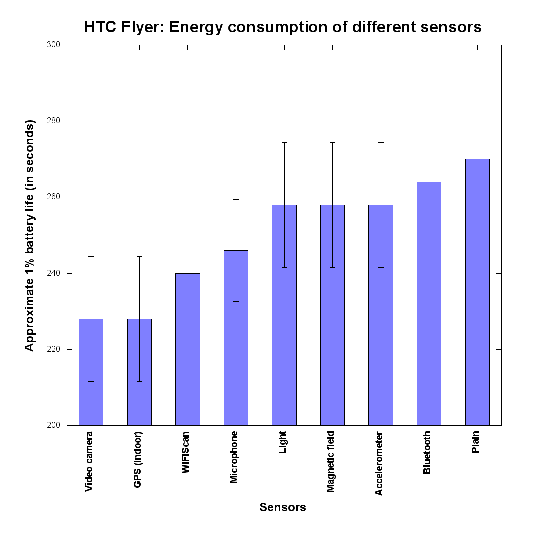
\includegraphics[width=0.49\textwidth, scale=0.6]{plots/htc_flyer}
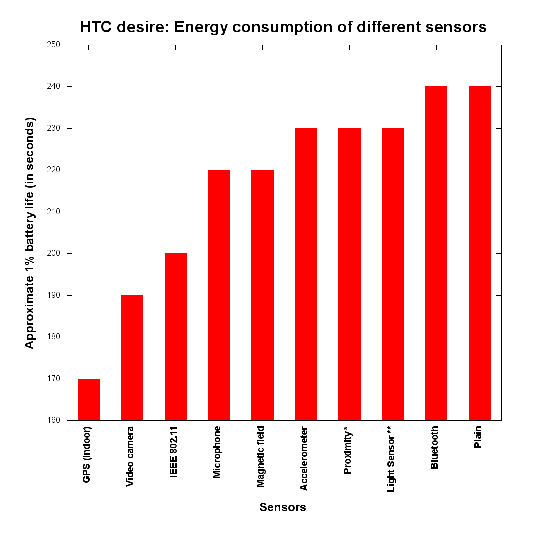
\includegraphics[width=0.49\textwidth, scale=0.6]{plots/htc_desire}
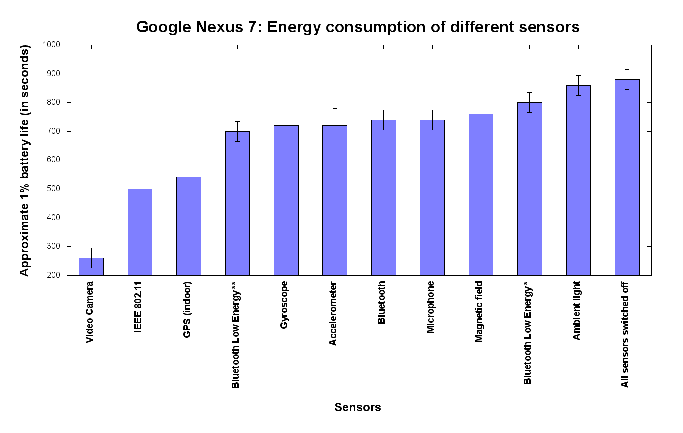
\includegraphics[width=\textwidth, scale=0.9]{plots/google_nexus_7}
\caption{\label{p:all_results} The complete results of energy measurements for all devices. The comparison of energy efficiency of different sensors is intuitive and overlaps with other research. }
\end{figure}

Bluetooth Low Energy\ (LE) may have higher energy demands than Classic Bluetooth. The figure (XXX-ref-bluetooth-le-api) compares their energy efficiency depending on the situation. In there is no device found, it takes longer for Bluetooth LE scanning to deplete the battery life by 1\% than for Classic Bluetooth scanning i.e. Bluetooth LE is more energy-efficient. However, if there is any device on the network, Bluetooth LE scanning depletes battery faster than Classic Bluetooth. The reason behind this phenomenon was analyzed in the previous section (the high output of Bluetooth LE API when any device is found) \ref{p:all_results}.
	
\plot{bluetooth_le_api}
				
The sensors energy efficiency order differs among the devices. The figure XXX-ref-to-the-figure contrasts the energy efficiency results for the shared sensors between the devices.For each of its diagrams, the order of the sensors on x axis is the same. The diagram on the left\ (Google Nexus 7) is characterized by monotonically increasing energy efficiency of the sensors, whereas the other two diagrams are not. For example, Bluetooth is the most energy efficient sensor HTC Desire and HTC Flyer, but is average for Google Nexus 7.
	
\begin{figure}[H]
\centering
\includegraphics[width=0.3\textwidth, scale=0.6]{plots/google_nexus_7_shared}
\includegraphics[width=0.3\textwidth, scale=0.6]{plots/htc_flyer_shared}
\includegraphics[width=0.3\textwidth, scale=0.6]{plots/htc_desire_shared}
\caption{\label{p:shared_sensors_results} Energy efficiency of shared sensors across different devices. The order of energy efficiency differs depending on a device. }
\end{figure}		
		
\subsubsection{Localization}

Different sensors may be used for localization purposes. The Figure (XXX-ref-all-locs) studies the energy efficiency of those sensors. For the comparison, the energy efficiency levels described in the previous section were used. For each of the devices, Bluetooth has the highest energy efficiency level i.e. it is the most energy-efficient. Also, microphone is always more energy efficient than traditional localization sensors\ (GPS and IEEE 802.11). On the other hand, the camera has worse energy performance than GPS and IEEE 802.11 on the two devices. Finally, the energy efficiency of GPS and IEEE 802.11 are similar, though WiFi scanning is more energy-efficient than GPS for two devices.  	

\plot{all_locs}

Physical sensors are more energy efficient than traditional localization sensors. The energy efficiency of accelerometer is compared with GPS and IEEE 802.11 scanning on the Figure (XXX-ref-acc-vs-loc). The accelerometer is more energy efficient, but the difference is not always substantial. For HTC Flyer and HTC Desire, the difference between the energy efficiency of accelerometer and traditional localization sensors is less than one energy efficiency level. It is worth reminding here that Accelerometer Sensor Application applies continuous sampling (i.e. sample as often as possible without sleeping intervals).
	
\plot{acc_vs_loc}		


\subsubsection{Conclusions}
The complete set of energy measurements' results are intuitive and overlap with other research, which uses different measurement methods [XXX references]. This gives validation to the energy measurement method used in this dissertation. For Google Nexus 7, the results confirm the energy-efficiency problems with Bluetooth Low Energy\ (API), which were noticed during the implementation phase. Finally, the energy measurement results vary among different devices. This justifies why the universal power model cannot be used. It also validates the necessity of online energy measurements. 

The analysis of the localization sensors' efficiency explains how localization technologies evolve. Bluetooth, the most energy efficient sensor, is already widely adopted in the industry. iBeacons (XXX reference), provided by Apple Inc.,  leverages Bluetooth LE for the indoor positioning system. Also, promising energy-efficiency results of microphone attracted research community. SurroundSenses \cite{azizyan:surroundsense} utilizes microphone for localization through ambient sound fingerprinting. Lastly, camera is the most expensive sensor, and thus, computer vision is not widely used for localization yet.
		
accelerometer cheaper localizations:
	this gives reason to leverage physical sensors for "expensive" sensors replacement
	accelerometer is still expensive
		reasons: IPC, continuous sampling
			it gives better functionality; is more complex; uses more energy
		result: smart sampling of physical sensors needs to be leveraged
			-validates why people do duty-cycling, adaptive sampling
			-our method did not deliver energy measurements based depending on those parameters^^
		this was shown before in XXX
		
Those results do not say anything on the cost when sensors are combined
		(crucial for providing some functionality out of physical sensors?)
		characteristics of cost? -> is it just CPU ?
			how WIFi and acceleromter vs wifi performs?
			how accelerometer and gyroscope vs acceleterometer performs?
				-intuition is that the result will not be much higher
			those questions are important for the idea behind  the library
				needs to be checked in practice separately.	
						
\subsection{Sensy}
\subsection{Conclusions}
	TODO ? summary previous conclusions
	
	complete set of results across three different phones including all sensors
		-believed that first such measurement
		
	the results which explain evolution of localization techniques
	
	Physical sensors:
		less expensive so can be leveraged for energy-efficient sensing
			-> validation for our library's design
		but provide more complex functionality, uses more energy
			require different strategies of using those "simple" sensors
				which gives a validation for movement detection in the library
		experiments does not say anything about combined values:
			how accelerometer+ wifi will be compared to acceleteremetor
				relevant for our energy-efficient library
	